\chapter{Introduction}

\drop{E}{arth} Observation (EO) commercial data sales have increased a 550\% in
the last decade \cite{sousa}[1]. This area is considered a key element in the
space industry and an opportunity market for the next years.

\acs{EO} industries implement on-premises conventional infrastructures to acquire,
store, process and distribute the geo-information generated.

However these solutions have the risks of over/under size the infrastructure, they are not flexible to cover sudden changes in the demand of services and the access to the information presents large latencies.  These aspects limit the use of \acs{EO} technology for real time use such as to manage crises, natural disasters and civil security among others (Deren, 2007).

In addition, new sectors and user typologies are applying for new \acs{EO} services
and there is an incresing demand of this services. These users
need more flexible, easy and instant access to \acs{EO} products and services through
the Web. This demand has traditionally been driven through Space Data
Infrastructures and heavy standards (ISO TC/211 and OGC) which are focused on
interoperability rather than the real demand from the end-users.

The use of cloud computing technology can overcome the previously defined limitations that present conventional infrastructures because of its elasticity, scalability and on-demand use characteristics (Armbrust, 2010).

GEO-Cloud Experiment goes beyond conventional data infrastructures used in \acs{EO}
industry and beyond the implementations of applications running in cloud, to
quest which parts of a complete infrastructure of \acs{EO} are technologically and
economically viable to be virtualized to offer basic and high added value
services (see Figure~\ref{fig:intr-geocloudConcept}).

\begin{figure}[!h]
\begin{center}
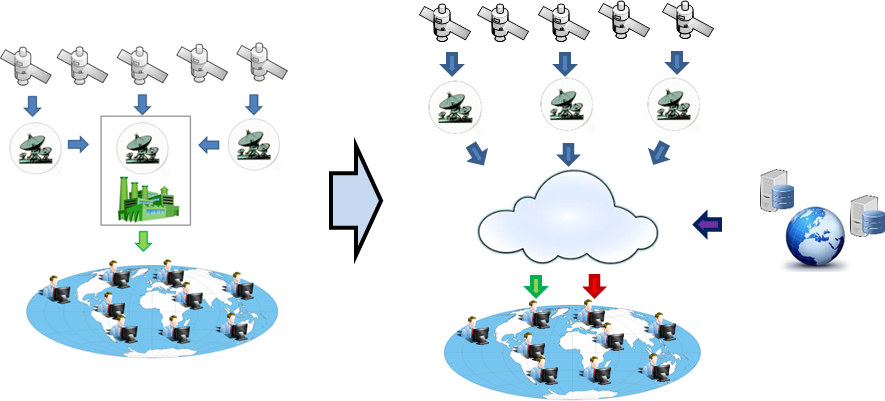
\includegraphics[width=0.6\textwidth]{statement/geocloudConcept.png}
\caption{The GEO-Cloud Concept. It is based on the use of cloud technology to acquire data, store it, process it, integrate it with other sources and distribute it to end users with the final objective of testing viable solutions for its real implementation.}
\label{fig:intr-geocloudConcept}
\end{center}
\end{figure}

GEO-Cloud  emulate the remote sensing mission with the satellites, the
topology network and the communications in the \vw testbed. The data
acquired from the emulated satellites is transferred to the \bonfire cloud
for storage, processing and distribution of data. End users accessing and
broadcasting will be emulated in another network implemented in \vw. In
order to implement realistic impairments in \vw, real networks will be
tested in \pl.  The technologies for imagery distribution and \acs{EO}
service delivery using cloud technologies and Internet protocols will be tested.

\section{The Geo-Cloud Experiment}

The GEO-Cloud experiment consists of the emulation of a realistic and complete Earth Observation System that provides services using cloud technology. For that purpose a constellation of satellites, ground stations, a cloud architecture, use cases and end users' models are designed.

The \acs{EO} system will be computed and emulated in \emph{Fed4FIRE}: A constellation of satellites record images of the Earth in a daily basis. The images are transferred to ground stations that ingest the data into a cloud computing infrastructure. The data is processed and distributed to end users.

The GEO-Cloud experiment is tested in three testbeds: \vw,\bonfire and
\pl. GEO-Cloud is divided into two sub-experiments:
\begin{itemize}
\item One experiment in a system integrated in \vw and \bonfire.
\item One experiment in \pl.
\end{itemize}

The experiment in \vw and \bonfire emulates the whole \acs{EO} system. In \vw:
constellation of satellites, the ground stations and the end users' models. In
\bonfire the cloud architecture, the processing chain of the data and its
distribution. Both \vw and \bonfire are interconnected to transfer information from one testbed to the other and viceversa.

The experiment in \pl consists of the emulation of the networks that constitute
the links between the ground stations to the cloud and from the cloud to the end
users. There, the network performance, features, bandwidth and impairments are
monitored and measured. Those parameters once measured are used to update the
models implemented in \vw, i.e, bandwidth, latency and loss rate.

In the next sections, the detailed design of the GEO-Cloud experiment is introduced.

\subsection{Satellite System Design}
\label{subsec:system-design}
\subsubsection{Design of the flight and ground segments}
\label{subsubsec:design-flight-ground}
In this subsection, the main characteristics of the system are presented. Objectives, constraints, previous estimations and possible modifications and their effects in the system are exposed.

In a wide vision, it is an \acs{EO} system consisting of a constellation of satellites equally spaced in a \acs{LEO} orbit with the aim of achieving daily coverage of the entire Earth surface. These conditions imply a very sophisticated handle of a huge quantity of data.

The following requirements have been fulfilled to design the system:
\begin{itemize}
\item Swath: $160km$ (based on state of the art cameras).
\item Resolution: $6.7m$ (based on state of the art cameras).
\item Low Earth Orbits.
\item Sun Synchronous orbits.
\item Download data rate: $160 Mbps$ (based on Deimos-2 satellite characteristics).
\item Optical Bands: 5 Multispectral (based on state of the art cameras).
\end{itemize}

\paragraph{Global Daily Coverage}~\\
The objective of this system is the acquisition of images of the total Earth surface in a daily basis. Global coverage is considered to include the land surface that is shown in Figure~\ref{fig:intr-land-surface}.


\begin{figure}[!h]
\begin{center}
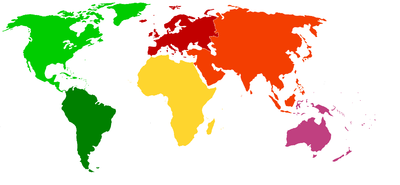
\includegraphics[width=0.6\textwidth]{detaildesign/surface-daily.png}
\caption{Land surface to be acquired in a daily basis}
\label{fig:intr-land-surface}
\end{center}
\end{figure}


\paragraph{Flight Segment}~\\
The satellites are selected according to the current state of the art. However,
some enhancements can be assumed as a way to adjust the analysis to the short
term future.


\subparagraph{Satellite performances}~\\
As a first iteration for the system, small platforms of less of $500kg$ are supposed according to the size and payload bay characteristics of representative platforms in this category. This study is based on the bus platforms currently offered by Surrey Satellite Technology Ltd, Satrec Initiative, Sierra Nevada Corporation, etcetera.

To reduce the amount of satellites orbiting the Earth, a design with two payloads has been assumed. Thus, the swath (the width of the field of view of each satellite in the surface of the Earth) can be duplicated without decreasing the resolution.

The satellites shall be pointing to nadir, acquiring images without maneuvering because of the acquisition plan for cover the Earth daily. Simultaneously, when a satellite gets into the field of view of a Ground Station, the download starts and at the same time the satellite continues imaging.

The main specifications of the satellites in the constellation are shown in Table~\ref{table:intro-satellite-performances}. The values of each parameter have been selected according to the state of the art and the desired quality of the images in the mission.

\begin{table}[hp]
  \centering
  {\small
  


\begin{tabular}{p{.2\textwidth}p{.2\textwidth}}
  \tabheadformat
  \tabhead{Specification}   &
  \tabhead{Value}\\
\hline
\textit{GSD}         & $6.7~m$ \\
\hline
\textit{Swath}         & $160~km$ \\
\hline
\textit{Number of bands}         & $5$ \\
\hline
\textit{Digitalization}         & $12~bits$ \\
\hline
\textit{Download Data Rate}         & $160~Mbps$ \\
\hline
\textit{Compression Rate}         &  $2:1$\\
\hline

\end{tabular}


% Local variables:
%   coding: utf-8
%   ispell-local-dictionary: "castellano8"
%   TeX-master: "main.tex"
% End:

  }
  \caption{Main Performances of the Satellites}
  \label{table:intro-satellite-performances}
\end{table}


\subparagraph{Orbit definition}~\\
It is common in \acs{EO} satellite missions the use of \emph{sun-synchronous} orbits. These orbits guarantee that the lighting conditions of the imaged places are the same during the mission, which is a very desirable characteristic.

\acs{LTAN} is also a desired condition of the orbit very related to the lighting and weather conditions of those places that the satellite overflies (\acs{LTAN} is selected according to the desired local time of the overflown places and the cloud formation during the day); it is common the use of \emph{LTAN 10:30h} for Earth Observation.

Other of the main parameters of an orbit is the altitude. Altitude has effects in the resolution and the swath of the satellites, which has impact in the number of satellites required to achieve the coverage objective. According to the value of those parameters in the payloads included in the satellites, the reference altitude for the system was found to be \emph{646km}. \acs{SSO} condition implies a relation between the altitude and the inclination of the orbit of \emph{97.97deg} in this case.

\subparagraph{Number of satellites in the constellation}~\\
The number of satellites shall be calculated using the altitude ($646 km$), the
inclination ($97.97 deg$) and a swath in
Table~\ref{table:intro-satellite-performances}. As a result, 17 satellites are
required to carry out this mission. In Figure~\ref{fig:intr-constellation-global} the whole constellation is
shown.

\begin{figure}[!h]
\begin{center}
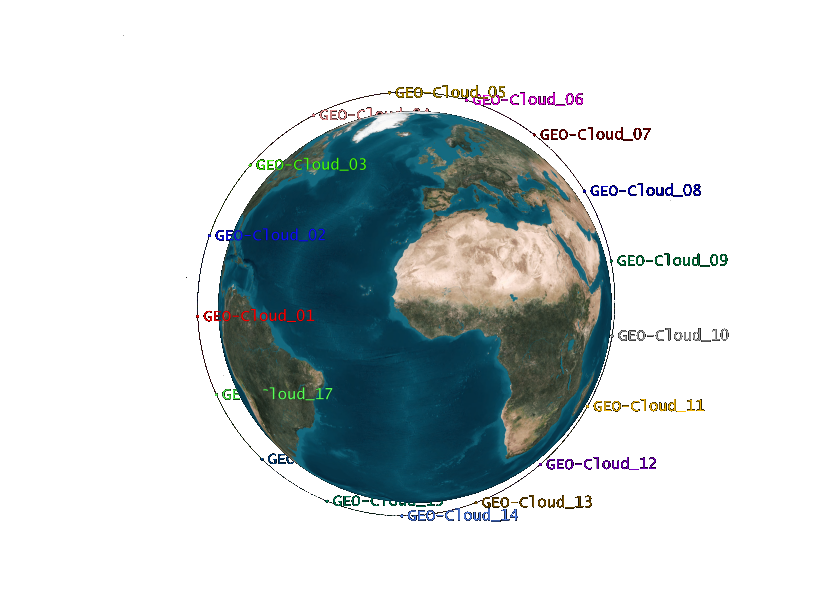
\includegraphics[width=0.6\textwidth]{detaildesign/constellation-global.png}
\caption{Constellation of 17 satellites in a SSO orbit at 646km}
\label{fig:intr-constellation-global}
\end{center}
\end{figure}

\paragraph{Ground Stations design}~\\
When the satellite acquires the data, it has to be downloaded to the Ground
Stations and then it has to be distributed to the customers. Due to the huge
quantity of data and the limitations the download data rate sets, several
stations distributed over the surface of the Earth are required. They will allow
the satellite to communicate with them and download the images. Due the
accumulated duration of the accesses to all the ground stations per day and the
frequency of accesses per day (it varies with the latitude of the station), the
Figure~\ref{fig:intr-footprints} shows how the Ground Stations and its
footprints (area in which the satellites can communicate with the Ground
Station) is distributed.


\begin{figure}[!h]
\begin{center}
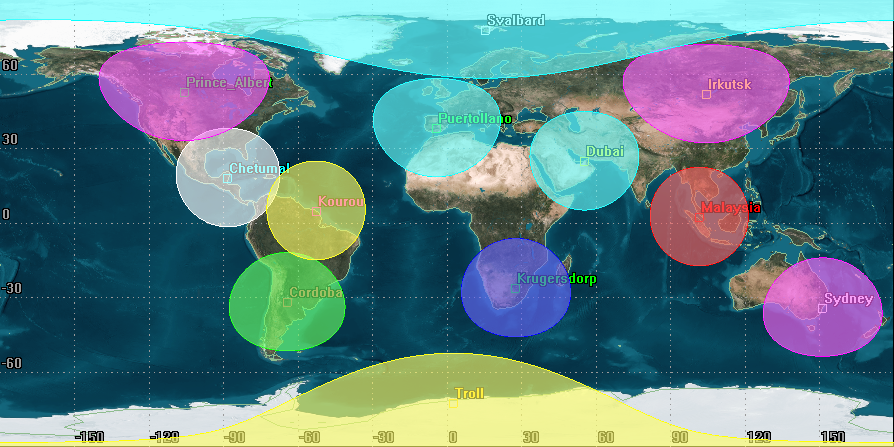
\includegraphics[width=0.8\textwidth]{detaildesign/footprints.png}
\caption{Footprints of the selected Ground Stations}
\label{fig:intr-footprints}
\end{center}
\end{figure}

\subsubsection{Generated Data Volume}

Specifically, $135,698,500 km^2$ of ground surface are daily acquired. With the following expression can estimate the data volume generated:

\begin{equation}
Acquired~Data~Volume= \frac{Acquired~Surface}{GSD^2} * Nº bands * Digitalization
\end{equation}

Before downloading the images they are compressed. The ancillary data is
included in the process (auxiliary information useful for the geolocation of the
images, protocol \ldots). In this case, the ancillary data is estimated to be
12\% of the acquired data (based on Deimos 2 satellite measurements), which is
added and then compressed. With the values depicted in
Table~\ref{table:intro-satellite-performances}, the ancillary and the daily ground
surface adquired, the data on ground can be estimated. As result including ancillary data before compression, \emph{11.55TBytes} shall be downloaded daily.


\subsection{Experiment Description}

The experiment consists of virtualizing a conventional \EO system to offer on
demand services to clients with the objective of validating its viability, find
the strengths and weaknesses of using cloud computing technology and establish
possible solutions for a future implementation in the market. There are three
components:
\begin{enumerate}
\item \emph{In-orbit mission:} this component generates the raw data. This consists of un-processed images of the Earth captured by a constellation of satellites and downloaded to different ground stations.
\item \emph{Treatment of data:} the data has to be stored, processed at different levels based on the services offered and distributed to the clients. The data acquired by the in-orbit mission is integrated with other sources to provide higher quality services.
\item \emph{End-users:} users of the provided services with different levels of remote access rights.

\end{enumerate}


\subsection{Experiment Design}


The GEO-Cloud experiment requires emulating a complete realistic Earth Observation Mission to provide high added value services such as crisis management. To this complex situation, the system has to response by processing on demand massive and variable amounts of stored and on line transferred data.

GEO-Cloud makes use of the following Fed4FIRE facilities: \pl,\vw and
\bonfire. \pl allows us to measure real network characteristics geographically
distributed to setup our models. \vw allows us to create any desired network
topology and emulate the in-orbit mission and the web service to the
users. \bonfire provides us a real cloud infrastructure with observability in
all the layers to test our cloud based services.


\paragraph{Implementation of the acquisition of geo-data in Virtual Wall and
  PlanetLab}~\\
The acquisition of geo-data is obtained from the in-orbit mission. The
constellation of satellites and the ground stations are emulated in \vw. A
network topology is implemented to communicate the different satellites with the ground stations. Every satellite in its orbit and every ground station models are simulated in a node.

The satellite models simulate the orbits and the pass of the satellites over the ground stations. The ground stations models simulate the coverture of the antennas and the download of the data. When a satellite is inside this radius, the satellite downloads the data to the ground station that is visible. The downloaded data in the ground stations is transferred to the \bonfire cloud.

With the \vw network,the \emph{bandwidths, latencies and loss rates} are
controlled.Also a realistic network topology to transfer data between different
nodes is created.

In order to determine the correct link characteristics for the connections
between the ground and the cloud infrastructure, a profilling tool has been
developed for measuring appropriate values for the link impairment between these different geographical locations using the \pl testbed.


\paragraph{Implementation of the cloud based services in BonFIRE}~\\
To facilitate offering the previous services we propose to implement a multi-layered cloud model in the \bonfire cloud infrastructure to generate on demand geo-information. The multi-layered cloud model is constituted of two layers:
\begin{itemize}
\item \emph{Layer 1:} This layer involves the basic satellite imagery services.  It acquires the raw data, stores it, has the first level of processing, distributes the processed data and offers the hosting service.

\item \emph{Layer 2:} This layer involves the high added value services. It can use historical processed, real time captured and pre-processed data from layer 1. This layer processes the information for real time generation of geo-information and offers real time access and distribution to the end-users. Typically, the implementation of high added value EO services involves the ingestion of the raster imagery from the satellites into a spatial database or storage, where it can be refined, simplified, processed or combined with other data sources in vector or raster format. The products, which can be vector or raster data, are distributed or queried using Internet technologies (OGC standards like WMS) or through Web services (tiles, caches, etcetera).
\end{itemize}

Thus, the whole EO system is completely implemented in Fed4FIRE, see Figure 3.

\begin{figure}[!h]
\begin{center}
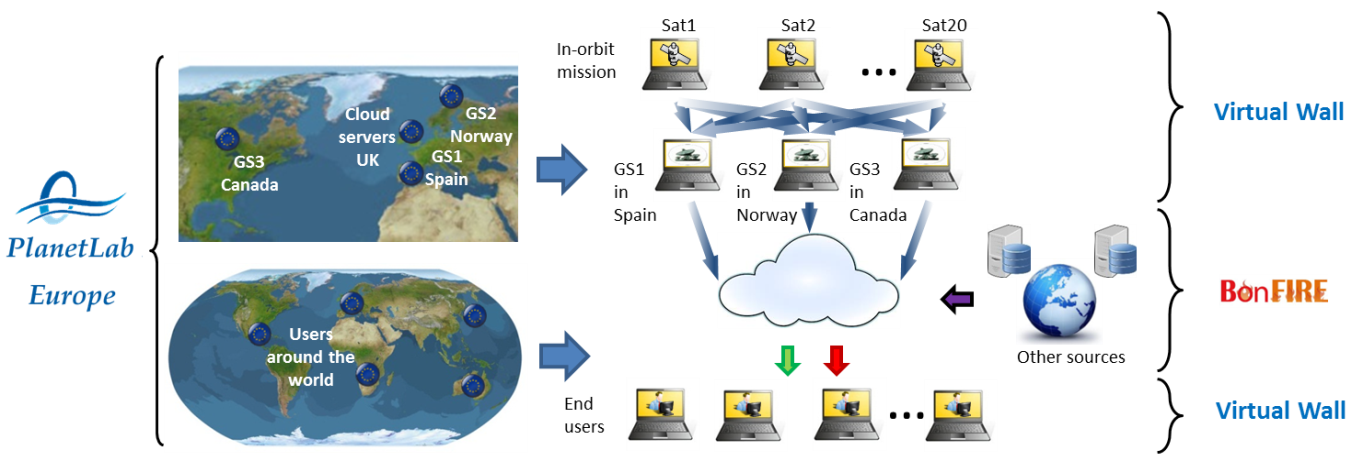
\includegraphics[width=0.6\textwidth]{statement/testbeds-geocloud.png}
\caption{Geo-Cloud implementation in Fed4FIRE}
\label{fig:intr-testbeds-geocloud}
\end{center}
\end{figure}


\subsection{Impact}

\subsection{Socio-Economical Impact Analysis}

The Geo-Cloud project is used as a framework to offer services from EO
users. The benchmark developed in the experiment allows to establish the
frontiers of viable and not viable cloud solutions in EO depending on

In the last decade, a large cantity of companies have started


\section{Scope of this end-career project}
Objetivos no???Por lo tanto esta seccion no es necesaria



\section{Document Structure}

Pueden incluirse aquí una sección con algunos consejos para la lectura del
documento dependiendo de la motivación o conocimientos del lector.  También
puede ser útil incluir una lista con el nombre y finalidad de cada uno de los
capítulos restantes.


\begin{definitionlist}
\item[Capítulo \ref{chap:antecedentes}: \nameref{chap:antecedentes}] Explica herramientas
  y aspectos básicos de edición con \LaTeX.
\item[Chapter \ref{chap:antecedentes}: \nameref{chap:objetivos}] In this
  chapter, the state of the art is showed and the differents studied tools and
  plattforms will be explained.
\item[Chapter \ref{chap:objetivos}: \nameref{chap:antecedentes}] Explica herramientas
  y aspectos básicos de edición con \LaTeX.
\item[Capítulo \ref{chap:objetivos}: \nameref{chap:objetivos}] Finalidad y justificación
  (con todo detalle) del presente documento.
\item[Capítulo \ref{chap:antecedentes}: \nameref{chap:antecedentes}] Explica herramientas
  y aspectos básicos de edición con \LaTeX.
\item[Capítulo \ref{chap:objetivos}: \nameref{chap:objetivos}] Finalidad y justificación
  (con todo detalle) del presente documento.
\end{definitionlist}
